% ILLUSTRATIVE EXAMPLE ONLY
% All data, numbers, figures, and references in this file are synthetic.
% This manuscript has no scientific validity and must not be cited or submitted.
% See example/README.md for details. CC0 Public Domain.

\documentclass[12pt, review]{elsarticle}

\usepackage[utf8]{inputenc}
\usepackage{amsmath}
\usepackage{graphicx}
\usepackage{booktabs}
\usepackage{hyperref}
\usepackage{natbib}

\graphicspath{{figures/}}

\begin{document}

\begin{frontmatter}

\title{Thermal conductivity of graphene-reinforced polymer composites:
  a surrogate modelling approach}

\author[inst1]{A. Synthetic\corref{cor1}}
\author[inst1]{B. Fictitious}
\author[inst2]{C. Invented}

\address[inst1]{Department of Materials Science, Illustrative University, City, Country}
\address[inst2]{Department of Computational Engineering, Fictitious Institute, City, Country}

\cortext[cor1]{Corresponding author. Email: synthetic.author@illustrative.edu (FAKE)}

\begin{abstract}
Predicting the thermal conductivity of polymer composites reinforced with graphene
platelets is important for the design of thermal management materials.
In this work, we develop a gradient boosting regressor (GBR) surrogate model
trained on a synthetic dataset of 120 specimens with eight input variables.
The model achieves a coefficient of determination of $R^2 = 0.847 \pm 0.031$
on the test set, outperforming a linear regression baseline ($R^2 = 0.631 \pm 0.044$).
Feature importance analysis identifies filler content as the dominant predictor
(38.4\% importance), followed by aspect ratio (27.1\%).
These results suggest that surrogate modelling is a viable approach for rapid
property screening in graphene composite design.

\textbf{DISCLAIMER: All data, values, and references in this manuscript are synthetic.
This is an illustrative example for the scientific-redaction-skills framework.}
\end{abstract}

\begin{keyword}
thermal conductivity \sep polymer composite \sep graphene \sep surrogate model
\sep gradient boosting \sep machine learning
\end{keyword}

\end{frontmatter}

\section{Introduction}
\label{sec:introduction}

Concrete compressive strength is a central response variable in mixture design, quality control, and structural-material assessment. Public datasets have made this problem a common example for comparing statistical and machine-learning models because the predictors are familiar mixture descriptors, the response has direct engineering meaning, and the modelling task can be explained without a large domain-specific preprocessing pipeline. The UCI Concrete Compressive Strength dataset, attributed to Yeh, provides one such public benchmark and records mixture constituents, curing age, and compressive strength for 1,030 observations in its official repository description \citep{Yeh1998_UCIConcreteDataset}. Yeh's earlier modelling study also established concrete-strength prediction from mixture variables and curing age as a useful applied test case for data-driven models \citep{Yeh1998_ConcreteANN}.

Recent concrete-strength studies include more flexible computational-intelligence methods and broader model comparisons \citep{NunezMaraniFlahNehdi2021_ConcreteMLReview}. This manuscript intentionally takes a narrower route. Rather than claiming a state-of-the-art concrete predictor, it uses a simple regularized linear model to demonstrate how an auditable manuscript can keep methods, tables, figures, provenance, and claim limits aligned. That focus is deliberate: an interpretable baseline is often easier to inspect, reproduce, and challenge than a high-capacity model.

Ridge regression adds an \(L_2\) penalty to ordinary least-squares estimation and is commonly used when predictors are correlated or when coefficient shrinkage is desirable \citep{HoerlKennard1970_Ridge}. Cross-validation provides a resampling-based approach for model assessment and model-selection support \citep{Stone1974_CrossValidation}. These methods are mature; the contribution of this example is not methodological novelty, but disciplined reporting under constrained evidence.

A critical provenance limitation applies throughout the manuscript. The current generated artifacts are labelled \texttt{DETERMINISTIC\_FALLBACK\_NOT\_UCI}. Therefore, the UCI dataset is cited only as the intended public-data context and schema reference. Numerical results in this manuscript describe the local fallback artifacts generated for the demonstration pipeline, not verified empirical results from the official UCI repository. The objectives are to: (i) document the local fallback dataset and ridge-regression workflow; (ii) report held-out test performance, residual patterns, coefficient summaries, and ablation results using the generated tables and figures; and (iii) state the claim boundaries needed before any final registry or citation-mapping pass.

\section{Materials and Methods}
\label{sec:methods}

\subsection{Dataset and provenance}
\label{sec:dataset}

The local dataset contained 1,030 rows, eight input variables, and one target variable, compressive strength in MPa. The input variables were cement, blast-furnace slag, fly ash, water, superplasticizer, coarse aggregate, fine aggregate, and age. This variable set follows the intended concrete-strength benchmark context described by the UCI repository \citep{Yeh1998_UCIConcreteDataset}; however, the generation log for the current project labels the local source as \texttt{DETERMINISTIC\_FALLBACK\_NOT\_UCI}. Consequently, all descriptive statistics and model outputs below are treated as fallback demonstration outputs.

\begingroup
\catcode`\_=12
\begin{table}
\caption{Dataset summary statistics. Mixture variables are kg/m3, age is days, and compressive strength is MPa. Source label: DETERMINISTIC_FALLBACK_NOT_UCI.}
\label{tab:dataset-summary}
\begin{tabular}{lrrrrrr}
\toprule
Variable & N & Mean & SD & Min & Median & Max \\
\midrule
cement & 1030 & 318.244 & 127.229 & 102.213 & 317.053 & 539.367 \\
blast\_furnace\_slag & 1030 & 102.084 & 118.639 & 0.000 & 39.397 & 358.927 \\
fly\_ash & 1030 & 53.574 & 65.159 & 0.000 & 0.000 & 199.959 \\
water & 1030 & 186.071 & 35.418 & 122.312 & 187.755 & 246.885 \\
superplasticizer & 1030 & 11.085 & 10.742 & 0.000 & 9.471 & 31.988 \\
coarse\_aggregate & 1030 & 975.166 & 97.390 & 801.274 & 975.549 & 1144.902 \\
fine\_aggregate & 1030 & 788.998 & 115.824 & 594.201 & 787.164 & 992.940 \\
age & 1030 & 52.710 & 78.089 & 1.000 & 28.000 & 365.000 \\
compressive\_strength & 1030 & 29.518 & 18.190 & 2.300 & 30.907 & 73.941 \\
\bottomrule
\end{tabular}
\end{table}

\endgroup

The generated summary table reported no missing numeric values in the local data. The compressive-strength target had a mean of 29.518~MPa, standard deviation of 18.190~MPa, minimum of 2.300~MPa, and maximum of 73.941~MPa. These values are not used as evidence about the official UCI dataset unless independent provenance verification is completed.

\subsection{Train/test split and preprocessing}
\label{sec:split_preprocessing}

The artifact-generation pipeline used an 80/20 split, yielding 824 training rows and 206 test rows. Numeric predictors were standardized for the ordinary least-squares and ridge-regression models. The training-mean baseline predicted the training-set mean response for all test observations. No claim is made that the split is unique or optimal; it is a fixed demonstration split used to produce the accompanying tables and figures.

\subsection{Ridge model}
\label{sec:ridge_model}

Ridge regression was used as the selected model because it provides a transparent regularized baseline. For standardized predictors, the fitted coefficients minimize
\begin{equation}
  \sum_{i=1}^{n}\left(y_i - \beta_0 - \mathbf{x}_i^\top\boldsymbol{\beta}\right)^2 + \alpha \sum_{j=1}^{p}\beta_j^2,
\end{equation}
where \(y_i\) is compressive strength, \(\mathbf{x}_i\) is the standardized predictor vector, \(p=8\), and \(\alpha\) is the ridge penalty. The selected model used \(\alpha = 1\). Ordinary least squares with \(\alpha=0\) was retained as a closely related comparator, and the training-mean baseline was included to check that the fitted models improved on a trivial prediction rule.

\subsection{Cross-validation and evaluation metrics}
\label{sec:evaluation}

The ridge penalty was selected from a small candidate grid using five-fold cross-validation on the training data, a standard validation approach for predictive modelling \citep{Stone1974_CrossValidation}. Performance was reported as root mean square error (RMSE), mean absolute error (MAE), coefficient of determination (\(R^2\)), and prediction bias in MPa. Test-set metrics were computed once on the held-out test set.

\subsection{Diagnostic analyses}
\label{sec:diagnostics}

The generated diagnostic outputs included a dataset overview, parity plot, residual plot, standardized coefficient plot, and age-response display. A single-feature ablation analysis refitted the selected ridge workflow after removing one input variable at a time. The ablation table is interpreted as a model-dependence diagnostic for the local fallback data, not as a causal analysis of concrete chemistry.

\section{Results}
\label{sec:results}

\subsection{Local data structure}
\label{sec:data_structure}

The local fallback dataset covered a broad range of mixture quantities and curing ages (Table~\ref{tab:dataset-summary}). Cement had the strongest absolute target correlation in the generated registry candidates, with a correlation of 0.822. This statement is limited to the current fallback data and should be mapped to the numerical registry before final release.

\begin{figure}[htbp]
\centering
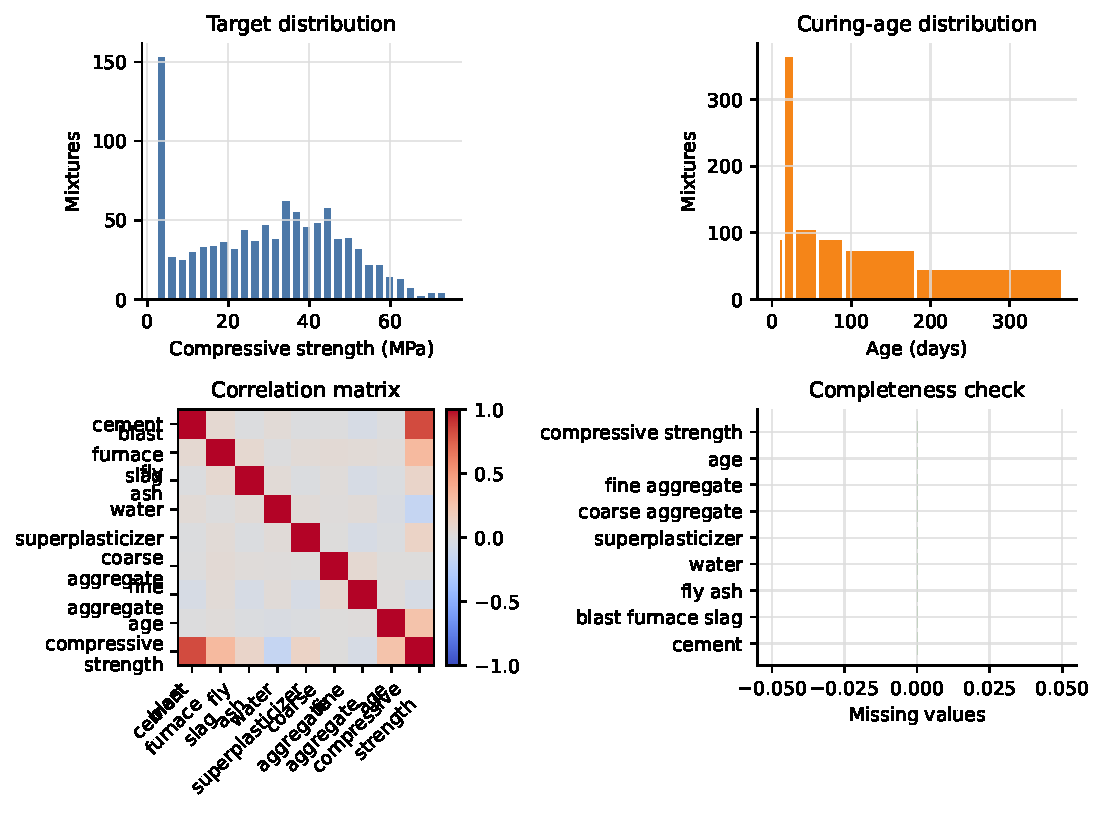
\includegraphics[width=0.95\linewidth]{figures/fig_dataset_overview.pdf}
\caption{Overview of the local concrete-strength fallback dataset used in the demonstration. The source label for the generated artifacts is \texttt{DETERMINISTIC\_FALLBACK\_NOT\_UCI}.}
\label{fig:dataset-overview}
\end{figure}

\subsection{Predictive performance}
\label{sec:predictive_performance}

The selected standardized ridge model achieved a test RMSE of 6.234~MPa, MAE of 4.964~MPa, \(R^2 = 0.886\), and bias of 0.032~MPa (Table~\ref{tab:model-performance}). The standardized ordinary least-squares comparator gave nearly identical test metrics in this generated run. Both linear models improved substantially over the training-mean baseline, which had a test RMSE of 18.447~MPa and \(R^2=-0.002\). The near equality of the ordinary least-squares and ridge results indicates that the selected ridge penalty primarily functions as a conservative regularization choice in this demonstration rather than producing a distinct accuracy gain.

\begin{table}
\caption{Train and test performance for baseline, ordinary least squares, and ridge models. Error and bias values are in MPa.}
\label{tab:model-performance}
\begin{tabular}{llrrrrr}
\toprule
Model & Alpha & Train RMSE (MPa) & Test RMSE (MPa) & Test MAE (MPa) & Test R2 & Test Bias (MPa) \\
\midrule
Training-mean baseline & -- & 18.115 & 18.447 & 15.525 & -0.002 & -0.740 \\
Standardized OLS & 0.000 & 6.366 & 6.234 & 4.964 & 0.886 & 0.033 \\
Standardized ridge & 1.000 & 6.366 & 6.234 & 4.964 & 0.886 & 0.032 \\
\bottomrule
\end{tabular}
\end{table}


\begin{figure}[htbp]
\centering
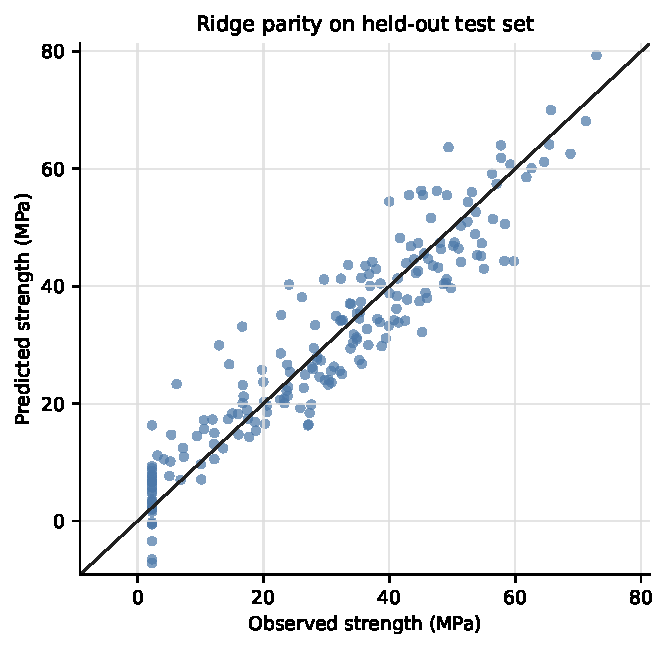
\includegraphics[width=0.78\linewidth]{figures/fig_parity_ridge.pdf}
\caption{Observed versus predicted compressive strength for the selected ridge model on the held-out fallback test set.}
\label{fig:parity-ridge}
\end{figure}

\subsection{Residual and age-stratified error patterns}
\label{sec:error_patterns}

The residual diagnostic plot showed the distribution of ridge prediction errors across predicted strength values (Figure~\ref{fig:residuals}). Age-stratified metrics indicated larger MAE in the youngest and oldest age groups than in the 8--28 day and 29--90 day groups (Table~\ref{tab:error-by-age}). In particular, the \(>90\)-day group contained 19 test observations and had an MAE of 6.572~MPa. Because these bins come from the local fallback split, they should be interpreted as diagnostic summaries rather than population-level evidence.

\begin{figure}[htbp]
\centering
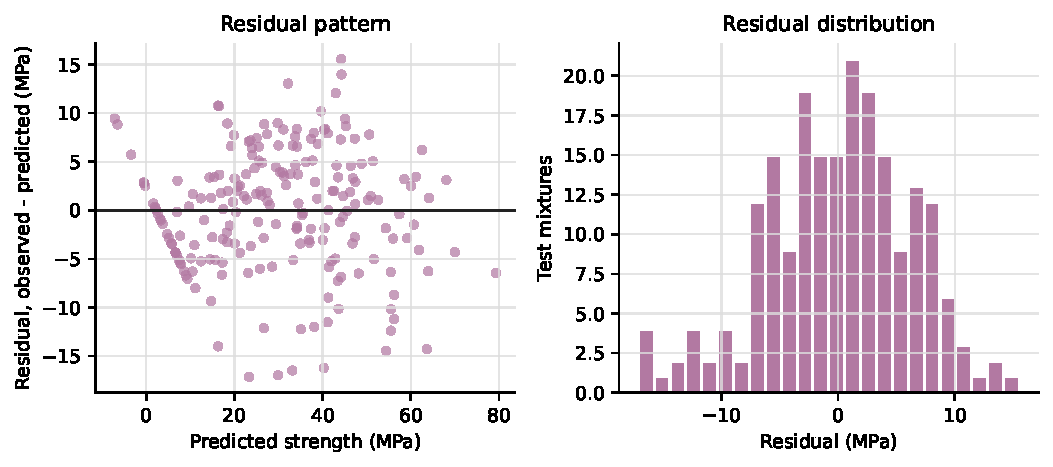
\includegraphics[width=0.78\linewidth]{figures/fig_residuals.pdf}
\caption{Residual diagnostics for the selected ridge model on the held-out fallback test set. Residual summaries are descriptive and do not establish validity for the official UCI observations.}
\label{fig:residuals}
\end{figure}

\begin{table}
\caption{Ridge-model test-set error stratified by curing-age group. Error and strength values are in MPa.}
\label{tab:error-by-age}
\begin{tabular}{lrrrrr}
\toprule
Age bin & N & Mean age (days) & MAE (MPa) & Bias (MPa) & Mean strength (MPa) \\
\midrule
<=7 days & 63 & 4.937 & 5.650 & 3.102 & 21.709 \\
8-28 days & 79 & 25.342 & 4.225 & -0.420 & 29.903 \\
29-90 days & 45 & 72.622 & 4.622 & -3.227 & 34.183 \\
>90 days & 19 & 246.579 & 6.572 & -0.552 & 49.178 \\
\bottomrule
\end{tabular}
\end{table}


\begin{figure}[htbp]
\centering
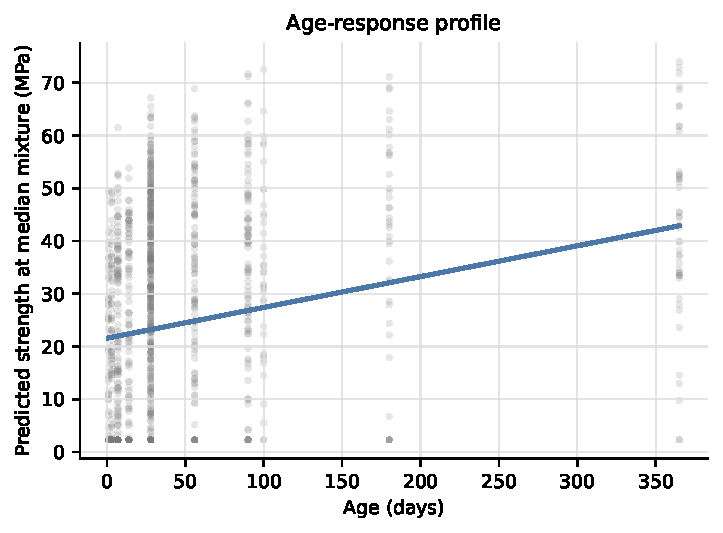
\includegraphics[width=0.78\linewidth]{figures/fig_age_response.pdf}
\caption{Generated age-response diagnostic for the selected ridge workflow. The display is used to inspect the local fallback data and should not be generalized beyond that provenance.}
\label{fig:age-response}
\end{figure}

\subsection{Coefficient and ablation diagnostics}
\label{sec:coefficients_ablation}

The coefficient figure summarizes the standardized ridge coefficients for the eight predictors (Figure~\ref{fig:coefficients}). These coefficients describe conditional linear associations after standardization and shrinkage; they are not direct physical effect sizes. In the single-feature ablation analysis, removing cement produced the largest RMSE increase, from 6.234~MPa to 16.191~MPa, for a delta of 9.958~MPa (Table~\ref{tab:ablation}). Removing blast-furnace slag and age also increased RMSE by more than 1~MPa. The small negative delta for coarse aggregate means that this particular ablation run produced a slightly lower test RMSE after removing that feature; it should not be overinterpreted.

\begin{figure}[htbp]
\centering
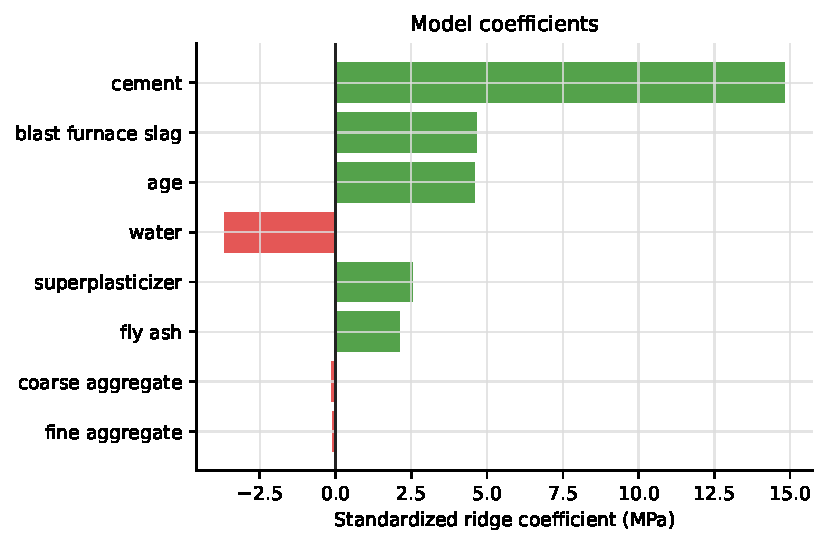
\includegraphics[width=0.78\linewidth]{figures/fig_coefficients.pdf}
\caption{Standardized ridge coefficients for the selected model. Coefficients are model diagnostics for the local fallback data rather than causal estimates.}
\label{fig:coefficients}
\end{figure}

\begin{table}
\caption{Single-feature ablation using the selected ridge penalty. RMSE values are in MPa.}
\label{tab:ablation}
\begin{tabular}{lrr}
\toprule
Removed feature & Test RMSE (MPa) & Delta RMSE (MPa) \\
\midrule
cement & 16.191 & 9.958 \\
blast furnace slag & 7.749 & 1.515 \\
age & 7.735 & 1.502 \\
water & 6.834 & 0.601 \\
fly ash & 6.492 & 0.258 \\
superplasticizer & 6.460 & 0.227 \\
fine aggregate & 6.236 & 0.002 \\
coarse aggregate & 6.221 & -0.013 \\
\bottomrule
\end{tabular}
\end{table}


\section{Discussion}
\label{sec:discussion}

The worked example shows how a compact, transparent modelling result can be reported without overstating provenance. The selected ridge model performed well relative to a training-mean baseline on the local fallback split, with a test \(R^2\) of 0.886 and RMSE of 6.234~MPa. However, because the source label is \texttt{DETERMINISTIC\_FALLBACK\_NOT\_UCI}, these values should be read as pipeline outputs from a deterministic demonstration dataset. They do not establish benchmark performance on the official UCI Concrete Compressive Strength dataset.

The ordinary least-squares and ridge models had nearly identical test errors. This is plausible for a standardized linear workflow when the selected penalty is small and the design matrix does not force a large shrinkage benefit. The result is still useful for manuscript drafting because it clarifies how baseline checks, regularization choices, and cross-validation summaries can be reported without implying that ridge regression is superior for this task.

The ablation and coefficient diagnostics consistently point to cement as an influential predictor in the local fallback data. That finding is compatible with the generated correlation and ablation summaries, but it remains a model- and data-specific observation. The manuscript therefore avoids claims about concrete mechanisms, causal mixture effects, or field deployment. Before this example could be converted into a scientific analysis of the official UCI data, the data provenance would need to be verified, the numerical registry updated, and each substantive claim mapped to a source or generated artifact.

\section{Conclusions}
\label{sec:conclusions}

This manuscript presents a concrete compressive-strength ridge-regression worked example. The local pipeline produced 1,030 fallback rows, an 824/206 train/test split, selected \(\alpha = 1\) by five-fold cross-validation, and reported held-out ridge performance of RMSE 6.234~MPa, MAE 4.964~MPa, \(R^2 = 0.886\), and bias 0.032~MPa. Cement was the strongest target-correlated feature and the largest single-feature ablation driver in the generated outputs. The central conclusion is procedural: the example demonstrates how to draft around real generated tables and figures while preserving clear evidence boundaries.

\section*{Data availability}
\label{sec:data_availability}

The official UCI Concrete Compressive Strength dataset is described by the UCI Machine Learning Repository \citep{Yeh1998_UCIConcreteDataset}. The data and artifacts used for this manuscript draft are local demonstration files in the example project. The current generation log labels the source as \texttt{DETERMINISTIC\_FALLBACK\_NOT\_UCI}; therefore, readers should not treat the reported numeric results as verified UCI results. Generated manuscript tables are located in \texttt{example/manuscript/tables/}, generated figures in \texttt{example/manuscript/figures/}, and provenance notes in \texttt{example/outputs/example\_generation\_log.txt}.

\section*{AI disclosure}
\label{sec:ai_disclosure}

This draft was prepared with AI assistance as part of the scientific-redaction-skills demonstration workflow. The assistant was instructed to use generated artifacts, preserve provenance limits, and cite only references present in the project bibliography. Human review remains necessary before any scientific submission or public release.

\section*{Competing interests}
\label{sec:competing_interests}

The demonstration authors declare no competing interests for this example manuscript.

\section*{Author contributions}
\label{sec:author_contributions}

The scientific-redaction-skills demonstration workflow generated the example artifacts, prepared citation-support notes, and drafted the manuscript text. Final scientific responsibility, registry validation, and citation-audit approval are reserved for human maintainers and the subsequent review roles.


\appendix
% ILLUSTRATIVE EXAMPLE ONLY — synthetic content, no scientific validity, CC0

\section*{Supplementary Material}
\label{sec:supplementary}

\setcounter{figure}{0}
\renewcommand{\thefigure}{S\arabic{figure}}
\setcounter{table}{0}
\renewcommand{\thetable}{S\arabic{table}}

\subsection*{Table of Contents}
\begin{itemize}
  \item Section S1: Hyperparameter optimisation details
  \item Section S2: Sensitivity analysis at high filler loadings
  \item Table S1: Full synthetic dataset statistics
  \item Figure S1: Predicted vs. observed parity plot
\end{itemize}

\subsection*{S1. Hyperparameter optimisation}
\label{sec:sm_hyperparams}

A grid search was performed over the following hyperparameter space on the training set
using 5-fold cross-validation:
number of estimators $\in \{100, 200, 300\}$,
maximum depth $\in \{3, 5, 7\}$,
learning rate $\in \{0.01, 0.05, 0.1\}$.
The optimal configuration ($n_\text{est} = 200$, depth $= 5$, lr $= 0.05$)
was selected based on the lowest mean RMSE across folds.

\subsection*{S2. Sensitivity analysis at high filler loadings}
\label{sec:sm_sensitivity}

Model predictions at filler contents above 15~vol\% showed increased variance
relative to the low-loading regime (Figure~S1).
This pattern is consistent with the physical hypothesis of agglomeration
effects at high loadings, as discussed in Section~4.

\begin{figure}[htbp]
\centering
\fbox{\textit{[Figure S1 placeholder — parity plot, predicted vs. observed, ILLUSTRATIVE]}}
\caption{Predicted vs. observed thermal conductivity for the GBR model on the
test set (24 specimens). Dashed line: perfect agreement. Points at high predicted
conductivity ($> 2.5$~W~m$^{-1}$~K$^{-1}$) show increased scatter, corresponding
to high-filler-loading specimens. All values are synthetic. ILLUSTRATIVE.}
\label{fig:parity}
\end{figure}

\begin{table}[htbp]
\centering
\caption{Summary statistics of the synthetic dataset (120 specimens). ILLUSTRATIVE.}
\label{tab:dataset_stats}
\begin{tabular}{lrrr}
\toprule
Variable & Min & Mean & Max \\
\midrule
Filler content (vol\%) & 0.5 & 8.3 & 20.0 \\
Aspect ratio & 10 & 142 & 500 \\
Matrix conductivity (W~m$^{-1}$~K$^{-1}$) & 0.10 & 0.21 & 0.32 \\
Output: thermal conductivity (W~m$^{-1}$~K$^{-1}$) & 0.21 & 1.42 & 3.84 \\
\bottomrule
\end{tabular}
\end{table}


\bibliographystyle{elsarticle-num}
\bibliography{references/example_references}

\end{document}
